\documentclass[10pt]{article}
\usepackage[polish]{babel}
\usepackage[utf8]{inputenc}
\usepackage[T1]{fontenc}
\usepackage{graphicx}
\usepackage[export]{adjustbox}
\graphicspath{ {./images/} }
\usepackage{amsmath}
\usepackage{amsfonts}
\usepackage{amssymb}
\usepackage[version=4]{mhchem}
\usepackage{stmaryrd}
\usepackage{hyperref}
\hypersetup{colorlinks=true, linkcolor=blue, filecolor=magenta, urlcolor=cyan,}
\urlstyle{same}

%New command to display footnote whose markers will always be hidden
\let\svthefootnote\thefootnote
\newcommand\blfootnotetext[1]{%
  \let\thefootnote\relax\footnote{#1}%
  \addtocounter{footnote}{-1}%
  \let\thefootnote\svthefootnote%
}

%Overriding the \footnotetext command to hide the marker if its value is `0`
\let\svfootnotetext\footnotetext
\renewcommand\footnotetext[2][?]{%
  \if\relax#1\relax%
    \ifnum\value{footnote}=0\blfootnotetext{#2}\else\svfootnotetext{#2}\fi%
  \else%
    \if?#1\ifnum\value{footnote}=0\blfootnotetext{#2}\else\svfootnotetext{#2}\fi%
    \else\svfootnotetext[#1]{#2}\fi%
  \fi
}

\begin{document}
\begin{center}

\includegraphics[max width=\textwidth]{2024_11_21_ddef65acdee69ef68bc2g-1}
\end{center}

\begin{enumerate}
  \item Dany jest czworokąt wypukły ABCD. Punkty K i L leżą odpowiednio na odcinkach AB i AD, przy czym czworokąt AKCL jest równoległobokiem. Odcinki KD i BL przecinają się w punkcie M. Wykaż, że pola czworokątów AKML i BCDM są równe.
  \item W trójkąt ostrokątny \(A B C\) wpisano kwadrat tak, że dwa jego wierzchołki należą do boku AB, a dwa pozostałe do pozostałych boków trójkąta. Udowodnij, że pole tego kwadratu nie przekracza połowy pola trójkąta \(A B C\).
  \item Trójkąt podzielono dwoma liniami na cztery części, jak na rysunku. Pola trzech z nich wynoszą 3, 6 i 4. Oblicz pole czwartej części.\\
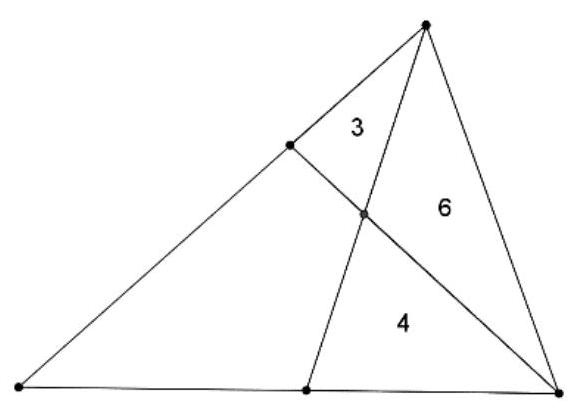
\includegraphics[max width=\textwidth, center]{2024_11_21_ddef65acdee69ef68bc2g-1(1)}
\end{enumerate}

\footnotetext{Rozwiazania nalė̇y oddać do piatku 1 marca do godziny 14.00 koordynatorowi konkursu panu Jarosławowi Szczepaniakowi lub przestać na adres \href{mailto:jareksz@interia.pl}{jareksz@interia.pl} do soboty 2 marca do pótnocy.
}
\end{document}